

\documentclass[11pt, a4paper]{article}
\usepackage[utf8]{inputenc}
\usepackage[T1]{fontenc}
\usepackage{lmodern}
\usepackage[margin=2cm]{geometry}
\usepackage{graphicx}
\usepackage{amsmath}
\usepackage{siunitx}
\usepackage[font=small, labelfont=bf]{caption}
\usepackage{titlesec}
\usepackage{enumitem}
\usepackage{cite}
\usepackage[hidelinks]{hyperref}

\titleformat{\section}{\large\bfseries}{\thesection}{0.6em}{}
\titleformat{\subsection}{\normalsize\bfseries}{\thesubsection}{0.5em}{}
\titlespacing*{\section}{0pt}{1.4ex plus 0.4ex minus 0.2ex}{0.6ex plus 0.2ex}
\titlespacing*{\subsection}{0pt}{1.0ex plus 0.3ex minus 0.2ex}{0.4ex plus 0.2ex}
\setlength{\parskip}{0.3ex}
\graphicspath{{figures/}}

\usepackage{xcolor}
\newcommand{\todo}[1]{\textcolor{red}{[TODO: #1]}}

\title{\textbf{Network inference in progressive MS stem cells:\\
a robust stress-signalling programme, an unresolved cholesterol route}}
\author{Sadegh Seyedhashemirizi\\Student ID i6427433\\[1ex]
\small Network Biology (MSc Systems Biology), Maastricht University}
\date{\today}

\begin{document}
% Title page (required: title, name, student ID, date, course name). Replace with the Canvas template if provided.
\begin{titlepage}
\centering
\vspace*{\fill}
{\Large\bfseries Network inference in progressive MS stem cells:\\
a robust stress-signalling programme, an unresolved cholesterol route\par}
\vspace{2.5em}
{\large Sadegh Seyedhashemirizi\par}
Student ID i6427433\par
\vspace{1em}
Network Biology (MSc Systems Biology), Maastricht University\par
\vspace{1em}
\today\par
\vspace*{\fill}
\end{titlepage}

% =====================================================================
\section{Introduction}
% =====================================================================

Network biology treats disease not as an isolated defect but as a perturbation that spreads
through networks of interacting molecules \cite{barabasi2011network}. Reconstructing such networks
from omics data follows two main paradigms. Data-driven methods learn patterns directly from the
measurements, for example co-expression networks \cite{huynhthu2010genie3} or factors shared across
omics layers \cite{argelaguet2020mofa,capraz2026sofa}, but they need large, sample-matched cohorts.
Prior-knowledge network (PKN) methods instead start from a curated map of known interactions and
ask which part of it best explains the changes measured in one condition. This step, called
contextualisation, turns a generic map into a cell-specific mechanistic hypothesis and remains
feasible with few samples \cite{garridorodriguez2022}.

PKN-based methods were developed separately for single biological layers. CARNIVAL fits signed
signalling paths to transcription factor (TF) activities \cite{liu2019carnival}, whereas iMAT and
flux balance analysis (FBA) fit metabolic flux under mass balance \cite{shlomi2008imat,orth2010fba}.
COSMOS joins signalling and metabolism, but does so by turning metabolic reactions into signed
edges \cite{dugourd2021cosmos}. CORNETO \cite{rodriguezmier2025corneto} recently framed all of these
as optimisation problems on a common hypergraph representation, which in principle allows them to be
solved together. In practice, however, the methods are still combined at a late level: they are
solved separately and compared or chained afterwards. A coupled signalling--flux model needs variables shared
where the layers meet, for example an enzyme's activity in the signalling model bounding the flux
of its reaction in the metabolic model, and such variables are not yet defined
(Fig.~\ref{fig:design}c). The structure of the inferred network depends on the PKN's edges, on which nodes may start a signal and on how
strongly small networks are preferred (Fig.~\ref{fig:design}b). How much of the inferred topology
comes from the data, and how much from the structure of the network itself, hasn't been thoroughly tested.

Progressive multiple sclerosis (PMS) is a useful test case, because Ionescu et al.\ combined several
omics layers with an explicit network hypothesis \cite{ionescu2024}. In induced neural stem cells
(iNSCs) from people with PMS, they found a senescent, neurotoxic state that the
cholesterol-synthesis inhibitor simvastatin reduced. They proposed a route from HMG-CoA reductase
(HMGCR) through cholesterol to six cholesterol-responsive TFs (E2F1, EGR1, WT1, SP1, JUN and JUNB).
Here we ask which TF activity changes distinguish PMS from control iNSCs, and whether
contextualisation, without being told where to start, recovers the proposed route
(Fig.~\ref{fig:design}a). We find a stress and senescence TF programme that is stable when any
line is left out, connected to a kinase layer that recurs across both PKNs, but no support for
synthesis-driven cholesterol signalling.

% =====================================================================
\section{Methods}
% =====================================================================

\subsection{Data and measured nodes}
We analysed public bulk RNA-seq of 3 control and 3 PMS iNSC lines (GSE297192
\cite{park2025,barrett2013geo}) together with metabolomics and lipidomics of 3 control and 4 PMS
lines (Metabolomics Workbench ST003331/ST003332/ST003328 \cite{ionescu2024,sud2016mw}). Replicates
were averaged, so that each cell line is one observation. Expression differences were scored with
a moderated $t$ statistic \cite{smyth2004limma}, and TF activities were inferred with CollecTRI
regulons and decoupler \cite{mullerdott2023collectri,badia2022decoupler}. The 50 most changed TFs,
all of which kept their sign when any one line was left out, became the measured signalling nodes.
The joint TF--metabolite fit added 36 metabolite contrasts, including free cholesterol. The RNA-seq that
Ionescu et al.\ analysed (2 vs 2 lines) comes from the same Park et al.\ study \cite{park2025}.
Because their raw proteomics are not public, their published table of 650 differentially abundant
intracellular proteins (adjusted $p<0.05$) served as an independent protein-level check.

\subsection{Networks and contextualisation}
The signalling PKN is OmniPath \cite{turei2021omnipath}, restricted to signed, directed, curated
edges between expressed genes (9,870 edges). The multi-omic PKN is COSMOS \cite{dugourd2021cosmos},
which adds Recon3D metabolic reactions \cite{brunk2018recon3d} and STITCH compound--protein
interactions \cite{szklarczyk2016stitch} (54,571 edges). CORNETO's CarnivalFlow selects the
subnetwork that best reproduces the measured signs, with a penalty $\lambda$ on the number of
edges. Any node without incoming edges may start a signal, with a sign chosen by the solver. To
avoid circularity, the nodes of the proposed route (HMGCR, SREBF1/2, SCAP, INSIG1, the six TFs,
mevalonate and cholesterol) were never allowed to start one. We fitted TFs alone on both PKNs, and a
joint TF--metabolite fit on COSMOS. Before any network was inspected, $\lambda$ was set to the largest
value that kept the fitting error within 10\% of the unpenalised ($\lambda=0$) fit.

\subsection{Testing what drives the inferred network}
\begin{itemize}[noitemsep, topsep=2pt, leftmargin=*]
  \item \emph{Is the route in the PKN?} We checked whether the reactions of the 20
        cholesterol-synthesis enzymes (KEGG \cite{kanehisa2000kegg}) connect in pathway order, and
        searched for the shortest HMGCR $\to$ cholesterol path while penalising hub metabolites
        \cite{croes2006weighted}. Pathway steps missing from COSMOS but present in Recon3D were
        restored in a repaired PKN.
  \item \emph{Can the method find it at all?} As a positive control, we fixed HMGCR as inhibited,
        with the simvastatin-induced fall in cholesterol as the only measurement.
  \item \emph{Data or network?} We refitted on ten degree- and sign-preserving randomised PKNs,
        under all 20 splits of the six RNA-seq lines into two groups, and with starting nodes
        restricted to receptors or with compound starting nodes removed.
  \item \emph{Which nodes are favoured?} We regressed whether an unmeasured node was selected on
        its $\log_2$ PKN degree (logistic regression) in real and randomised networks, and ranked
        recurring nodes by degree and betweenness.
  \item \emph{Does mass balance change the answer?} We built Recon3D (10,600 reactions) in CORNETO
        and fitted iMAT models \cite{shlomi2008imat} to the group-mean expression (top and bottom
        quartiles as high and low). Uptake was allowed for compounds detected in no-cell medium
        blanks, plus cholesterol, which the B27 supplement of the culture medium contains. FBA
        \cite{orth2010fba} then gave each model's capacity to make cholesterol with and without
        uptake.
  \item \emph{Integration style.} We compared a metabolite-only fit merged afterwards with the
        TF-only fit (late integration) against the joint TF--metabolite fit on COSMOS, in which
        both layers are solved in one network problem (intermediate integration). Neither is early integration,
        which would combine matched samples before modelling: our layers come from different
        experiments.
\end{itemize}
Fits were solved as mixed-integer linear programs with HiGHS \cite{huangfu2018highs} in CORNETO
1.0.0rc8, for $\lambda$ = 0, 0.01, 0.03, 0.1, 0.3 and 1, with a 1\% optimality gap and 30--60\,min
time limits. Overlaps are Jaccard
indices. Code, settings and input checksums are in the project repository.

% =====================================================================
\section{Results}
% =====================================================================

\subsection{A stress TF programme, a recurring kinase layer, and HMGCR raised only as protein}
PMS lines activated a stress and senescence programme: SP1 and JUN ranked second and sixth of 628
TFs and the AP-1 and NF-$\kappa$B complexes 13th and 25th (Fig.~\ref{fig:tf}a), while JUNB and EGR1
rose moderately, E2F1 was unchanged and WT1 is not expressed. In all three fits, the kinases MAPK1,
MAPK14 (p38$\alpha$), PRKACA, FYN and AKT1 sat directly upstream of these TFs
(Fig.~\ref{fig:network}a), although the networks shared only 7--21\% of their edges; all five are
among the top 1\% of OmniPath proteins by degree. Sterol-synthesis genes were not induced
(Fig.~\ref{fig:tf}b), but HMGCR protein was about nine-fold higher in PMS lines (adjusted
$p=2\times10^{-6}$), although protein and mRNA changes otherwise agreed (Spearman 0.51 over 606
genes).

\subsection{The cholesterol route is in the network but is not selected}
The synthesis pathway is in COSMOS except for one step (squalene synthase, FDFT1), which we
restored in a repaired PKN. With HMGCR fixed as inhibited and the simvastatin-induced fall in
cholesterol as the only measurement, CarnivalFlow recovered the canonical route in the repaired PKN
but took a 32-edge mitochondrial detour in the original (Fig.~\ref{fig:aim5}a). From the PMS data
alone, neither fit used synthesis: a single Golgi-to-cytosol transport step explained the
cholesterol rise (Fig.~\ref{fig:aim5}b), and about 480 other metabolites are as close to SP1 as
cholesterol is. The mass-balanced iMAT/FBA models agreed: control and PMS had the same active
synthesis pathway, and when uptake was allowed neither required synthesis.

\subsection{What the network contributes}
The inferred networks were strongly sensitive to PKN structure and to the choice of starting
nodes. First,
\emph{hubs are favoured}: each doubling of an unmeasured node's PKN degree raised its odds of
selection 1.7- to 3-fold, to the same extent in randomised networks (Fig.~\ref{fig:robust}c).
Second, \emph{a good fit is not evidence for the topology}: six of ten randomised PKNs fitted every
TF sign exactly, while sharing only 7--18\% of inferred nodes with the real network. Third,
\emph{one starting node dominates, but which one is arbitrary}: a single starting node sat upstream
of 24--92\% of the explained measurements, and its identity changed with $\lambda$ and PKN
(Fig.~\ref{fig:robust}a). In the joint TF--metabolite fit it was an unmeasured tamoxifen node,
upstream of 39 of the 79 measurements that are reachable in the network (Fig.~\ref{fig:network}).
Restricting starting nodes to receptors gave the same pattern, with one receptor (PTPRE) upstream
of 49 of 50 TFs, and removing compound starting nodes moved the dominance to a single protein hub.
The data nevertheless carry signal: of all 20 ways to split the six lines into two groups, only the
true grouping and its mirror image were fitted without error ($p=2/20$).

% =====================================================================
\section{Discussion}
% =====================================================================

The stress TF programme and its kinase layer fit the senescent phenotype: p38 MAPK and NF-$\kappa$B
drive the senescence-associated secretory phenotype \cite{freund2011p38,chien2011nfkb}, and AP-1
organises the senescence transcriptional programme \cite{martinezzamudio2020ap1}. The raised HMGCR
protein without transcriptional induction could reflect reduced INSIG-dependent degradation
\cite{deboseboyd2008feedback}, which was not measured here. Every method in this study reads HMGCR only
through its mRNA, so this possible entry point of the proposed route was invisible to them, and the
network results neither confirm nor refute it.

More broadly, contextualisation could not settle the question because of four properties of
PKN-based inference:
\begin{enumerate}[noitemsep, topsep=2pt, leftmargin=*]
  \item \textbf{Identifiability.} With thousands of candidate starting nodes, the edge penalty
        collapses the solution onto a single hub, and many hubs work equally well. The data
        constrain the last step into the TFs, not the path before it, which is why randomised
        networks fit as well as the real one.
  \item \textbf{Hub bias.} Selection favours high-degree nodes even in randomised networks, so
        recurrence alone, as for the kinase layer, does not establish biological involvement.
  \item \textbf{PKN completeness.} A single missing reaction (FDFT1) hid a textbook pathway, and
        nothing in the network signals such a gap.
  \item \textbf{Signs are not chemistry.} In a signed network, an active enzyme ``produces'' its
        product without consuming anything, so one transport edge explains a rise in cholesterol
        as well as the whole synthesis pathway does. A stoichiometric model forbids this, because
        every molecule must be made or taken up, but without measured uptake rates it still cannot
        tell synthesis from uptake.
\end{enumerate}

\paragraph{Integration styles.}
We tried late integration (TF and metabolite networks fitted separately and merged) and
intermediate integration (the joint TF--metabolite fit); neither placed a measured metabolite
upstream of a TF. Connecting the signalling and metabolic models through shared constraints, such
as an enzyme's inferred activity bounding the flux of its reaction, remains future work, which
CORNETO's common framework makes possible.

\paragraph{Next steps.}
Four changes would make the upstream part of such networks testable. First, starting nodes should
be limited to measured perturbations, for example simvastatin treatment or ligands detected in the
secretome, instead of every source node in the PKN. Second, enzyme activity should enter at the
protein level: the HMGCR increase seen here only in proteomics could then be a measured node rather
than an inferred one. Third, CarnivalFlow and iMAT should be coupled in one CORNETO problem, so that
an inactive enzyme forbids flux through its reaction and measured uptake and secretion from the
spent medium bound the exchanges. Fourth, every inferred node should be compared with
degree-matched null nodes, for example cholesterol against random metabolites of similar degree as
a starting node, so that hub recurrence is not mistaken for evidence. Profiling the same cell lines
in every layer would, in addition, allow factor models and PKN methods to be compared on equal
terms.

\paragraph{Conclusion.}
The public PMS data support a stress and senescence TF programme and, at the protein level, a
raised HMGCR. Network contextualisation cannot resolve whether HMGCR acts through cholesterol on
these TFs: the step is invisible to mRNA-based inputs, and the upstream network is shaped by hubs
and by the choice of starting nodes rather than by the data. Measured HMGCR activity, isotope
tracing into cholesterol combined with a TF readout, or knockdown of the candidate TFs under
simvastatin would distinguish the competing explanations.

% =====================================================================
% FIGURES (excluded from the 3-page text limit)
% =====================================================================
\clearpage

\begin{figure}[htbp]
  \centering
  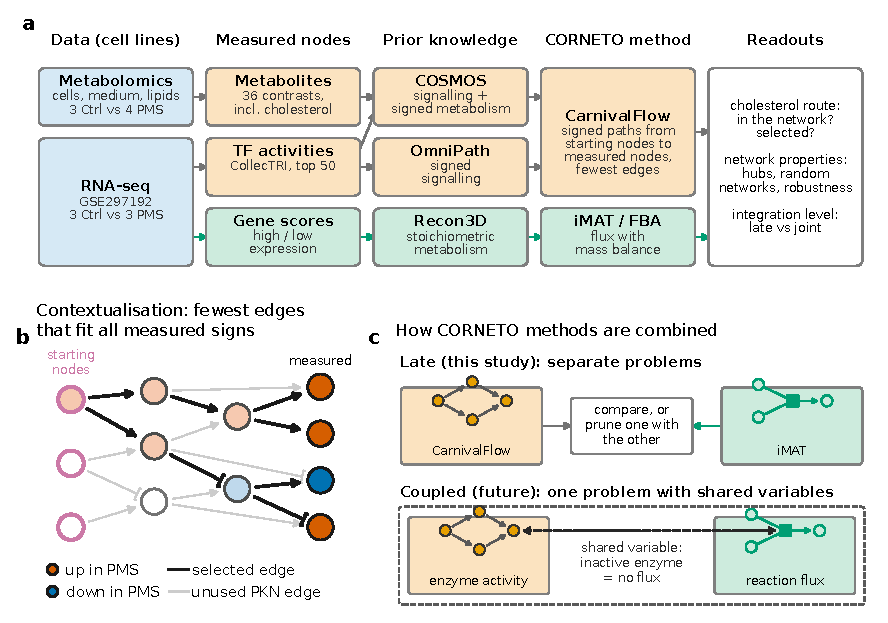
\includegraphics[width=\textwidth]{fig1_concept.pdf}
  \caption{\textbf{Data, networks and how the CORNETO methods were combined.} (a) Workflow.
  Metabolomics and lipidomics: Metabolomics Workbench ST003331 (cells), ST003332 (medium) and
  ST003328 (lipids, with a simvastatin arm). The PKNs are OmniPath (9,870 edges), COSMOS (54,571
  edges) and Recon3D (10,600 reactions). Orange: signed networks and CarnivalFlow; green:
  stoichiometric metabolism and iMAT/FBA. (b) Contextualisation, toy example. Signals may start at
  nodes without incoming edges (pink outline). CarnivalFlow keeps the fewest PKN edges whose signs
  reproduce every measured node; light colours are inferred states. (c) In this study the signed
  and stoichiometric methods were solved separately and combined afterwards (late). A coupled model
  would solve both in one problem, linked by shared variables such as an enzyme's activity
  bounding the flux of its reaction.}
  \label{fig:design}
\end{figure}

\begin{figure}[htbp]
  \centering
  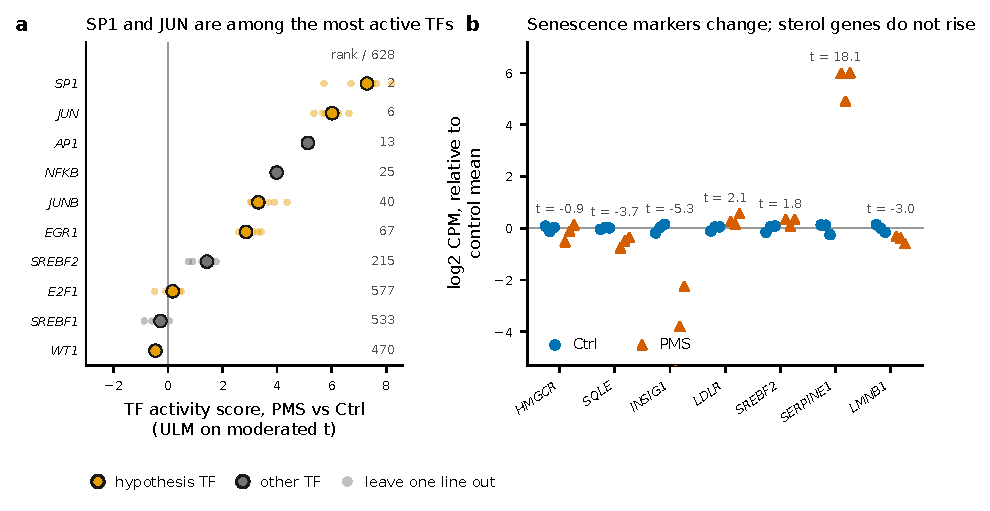
\includegraphics[width=\textwidth]{fig2_tf_activity.pdf}
  \caption{\textbf{PMS lines show a stress TF programme without induction of sterol synthesis
  (3 vs 3 lines).} (a) TF activity scores for the six hypothesis TFs (orange), the SREBFs and the
  AP-1/NF-$\kappa$B complexes. Large dots: all lines; small dots: leaving out one line; numbers:
  rank among 628 TFs. Activity scores are inferred from each TF's target genes; WT1 itself is not
  expressed, so its score is not interpretable. (b) Per-line expression relative to the control mean, with the moderated
  t statistic. Senescence markers change, while sterol-synthesis genes do not rise.}
  \label{fig:tf}
\end{figure}

\begin{figure}[htbp]
  \centering
  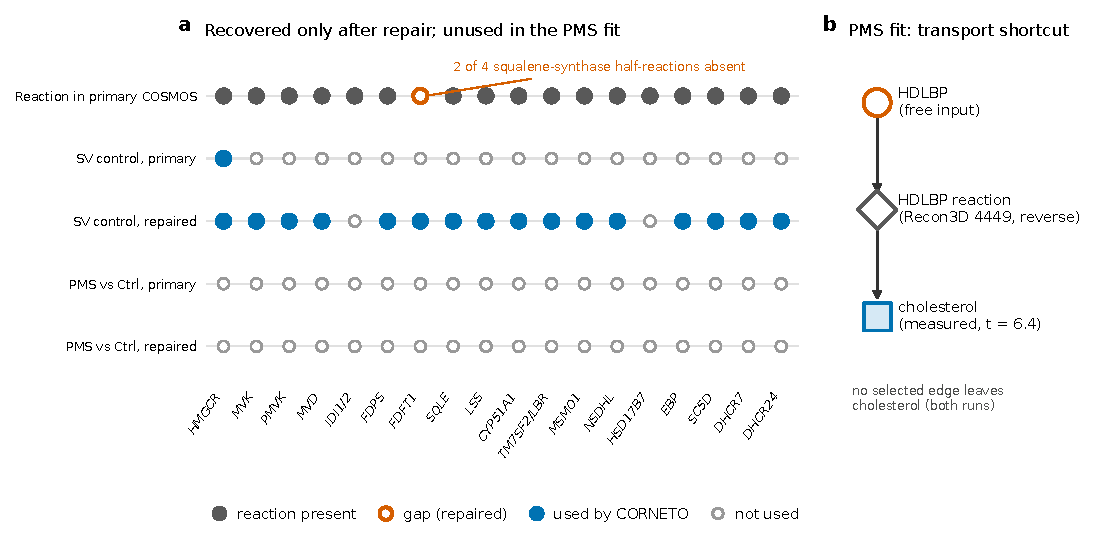
\includegraphics[width=\textwidth]{fig3_aim5_route.pdf}
  \caption{\textbf{The cholesterol route is in the network but is used only for a known
  perturbation.} (a) The cholesterol-synthesis enzymes in pathway order. Row 1: present in COSMOS;
  the two squalene-synthase (FDFT1) half-reactions are missing and were restored in the repaired
  network. Rows 2--3: enzymes used when CORNETO was told that HMGCR is inhibited and cholesterol
  falls (simvastatin), in the original and the repaired network; in the original network the
  solver reached cholesterol by a 32-edge detour through unrelated mitochondrial reactions. Rows
  4--5: enzymes used in the PMS-versus-control fits. (b) In both PMS fits, the cholesterol rise is
  explained by one Golgi--cytosol transport step.}
  \label{fig:aim5}
\end{figure}

\begin{figure}[htbp]
  \centering
  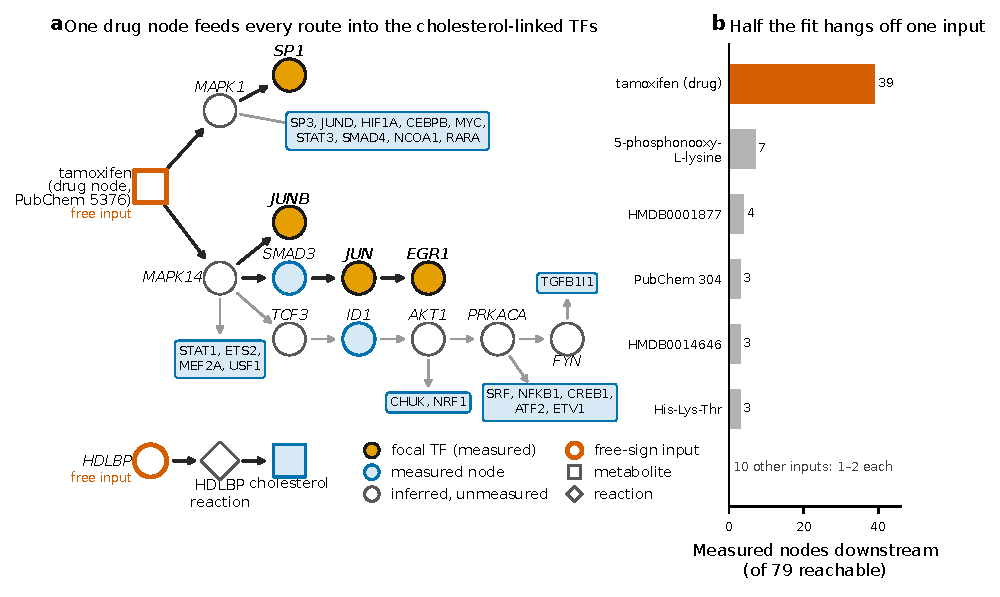
\includegraphics[width=\textwidth]{fig4_cosmos_subnetwork.pdf}
  \caption{\textbf{A kinase layer connects to the cholesterol-linked TFs in the joint
  TF--metabolite fit.} The fit on COSMOS ($\lambda=0.1$), restricted to the routes into SP1, JUNB,
  JUN and EGR1. (a) All routes pass through the kinases MAPK1 or MAPK14 and start at one unmeasured
  starting node, a tamoxifen compound; no route starts from cholesterol. Blue boxes collapse further
  measured TFs. All shown nodes are inferred as increased in PMS. (b) Measured nodes downstream of
  each starting node used, out of the 79 measurements reachable in the network (all 50 TFs and 29
  of the 36 metabolites).}
  \label{fig:network}
\end{figure}

\begin{figure}[htbp]
  \centering
  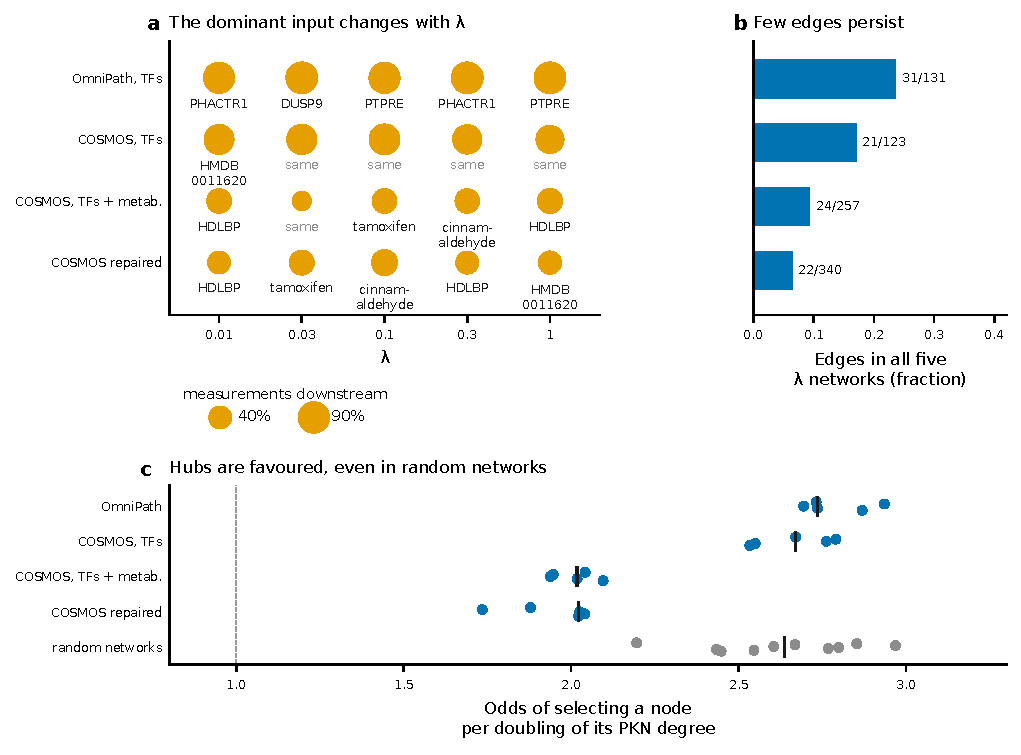
\includegraphics[width=\textwidth]{fig5_robustness.pdf}
  \caption{\textbf{What changes, what persists, and why.} (a) For each fit and penalty $\lambda$,
  the starting node upstream of the most measurements (dot area: fraction of measurements;
  ``same'': unchanged from the previous $\lambda$). (b) Edges selected at all five $\lambda$
  values, as a fraction of all edges ever selected. (c) Odds that an unmeasured node is selected, per doubling of its PKN
  degree (logistic regression; dots: $\lambda$ values or random networks; bars: medians).
  Selection favours hubs to the same degree in degree-preserving random networks.}
  \label{fig:robust}
\end{figure}

\clearpage
\bibliographystyle{unsrt}
\bibliography{references}

\end{document}
